\scanpage{13}

% 1, upper left
1) \quad $F_0$

% 2, first diagram
\diagram{\begin{tikzcd}[ampersand replacement=\&,column sep=small,row sep=small]
\&R_1\arrow[dl]\arrow[dr,"\text{épi}"]\\
2)\ F_0\&\&F_1
\end{tikzcd}}

% 3, cancelled first attempt
\diagram{\begin{tikzcd}[ampersand replacement=\&,column sep=tiny,row sep=tiny,execute at end picture={\draw[thick] (\tikzcdmatrixname-1-2.west) -- (\tikzcdmatrixname-2-1.west) -- (\tikzcdmatrixname-1-2.east) -- (\tikzcdmatrixname-3-1.east) -- (\tikzcdmatrixname-2-3.north) -- (\tikzcdmatrixname-3-3.west);}]
\&\deleted{R'_1}\arrow[dl]\arrow[dr,"\deleted{\text{épi}}"]\\
3)\ \deleted{F'_0}\arrow[d]\&\deleted{R_1}\arrow[dl]\arrow[dr,"\deleted{\text{épi}}"]\&\deleted{F'_1}\arrow[d]\\
F_0\&\&F_1\&F_2
\end{tikzcd}}

% 3, second drawing beside crossed version
\diagram{\begin{tikzcd}[ampersand replacement=\&,row sep=small,column sep=small]
\& R'_1\arrow[dl,very thick]\arrow[dr,two heads]\arrow[dd,very thick]\arrow[dddrr,dashed]\\
F'_0\arrow[dd,very thick]\arrow[ddrrr,dashed]\&\& F'_1\arrow[dd,very thick]\arrow[ddr]\\
\&R_1\arrow[dl]\arrow[dr,two heads]\\
F_0\&\&F_1\&F_2
\end{tikzcd}}

% top right, decomposition and list
décomposition cellulaire \deleted{drapeaux} \inserted{correspond : l'ens} \deleted{\unsure{complexe simplicial|quasi-simplicial} sommets $=F_0\amalg F_1$} ordonné des drapeaux
\[
\begin{aligned}
\text{type }0 &:F_0\\
\text{type }1 &:F_1\\
\text{type }(0,1)&:R_1
\end{aligned}
\]

% top right, marked points and loops
\figure{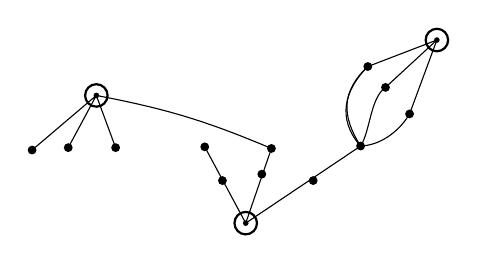
\begin{tikzpicture}[x=1.02cm,y=1.02cm]
\coordinate (a) at (.8,1.25); \coordinate (b) at (2.66,-.34); \coordinate (c) at (4.09,.62); \coordinate (d) at (5.04,1.94);
\draw (0,.57)--(a)--(.45,.6) (a)--(1.04,.6) (a) to[bend left=6](2.98,.59)--(b)--(2.15,.61) (b)--(c);
\draw (c)..controls (3.79,.96) and (3.89,1.32)..(4.18,1.61)--(d);
\draw (c)..controls (3.85,1) and (3.85,1.3)..(4.18,1.61);
\draw (c)..controls (4.21,.8) and (4.21,1.22)..(4.4,1.35)--(d);
\draw (c)..controls (4.36,.63) and (4.59,.83)..(4.7,1.02)--(d);
\foreach \p in {(0,.57),(.45,.6),(1.04,.6),(2.15,.61),(2.37,.19),(2.86,.27),(2.98,.59),(3.5,.19),(c),(4.18,1.61),(4.4,1.35),(4.7,1.02)}{\fill \p circle(.055);}
\foreach \p in {a,b,d}{\draw[thick](\p)circle(.14); \fill(\p)circle(.035);}
\end{tikzpicture}}

% 4, below left
4) \qquad $F_0$

% 4, below the isolated F
\diagram{\begin{tikzcd}[ampersand replacement=\&,row sep=small,column sep=small]
\& R'_1\arrow[dl,very thick]\arrow[dr,two heads]\arrow[dd,very thick]\arrow[dddrr,dashed]\\
F'_0\arrow[dd,dash]\arrow[ddrrr,dashed]\&\& F'_1\arrow[dd,very thick]\arrow[ddr]\\
\&R_1\arrow[dl]\arrow[dr,two heads]\\
F_0\&\&F_1\&AF_2
\end{tikzcd}}

% lower left, initial categories
$\deleted{C_0=\unsure{\mathrm{Ens}_f|\mathrm{Ens} f}}$

$C_1={}$

% lower half, definition of family category
$\Phi(C)={}$ Catégorie des \deleted{\unsure{couples|triples}} \deleted{\unsure{$I,$}} \inserted{familles finies} $\{(f_i)_{i\in I}\}$ de morphismes de $C$ de \unsure{$=$|m\textsuperscript{e}} but \deleted{\unsure{$I$, ens. fin.}}

% below definition, induced functor
Un foncteur $C\xrightarrow{\unsure{r|\varphi}}(\mathrm{Top}\ \deleted{\unsure{isotop.}})$ implique un foncteur
\[
 \begin{aligned}
 \Phi(C)&\xrightarrow{\deleted{\unsure{\varphi}}\Phi(r)}\mathrm{Top}\\
 (X_i\overset{\unsure{f_i}}{\to} X)_{i\in I}&\longmapsto
 \coprod_i\underbrace{\operatorname{cône}}_{\mathord{\hookrightarrow}}\deleted{\unsure{F|\varphi}}r(X_i)
 \underset{\coprod\Phi(X_i)}{\amalg}r(X)
 \end{aligned}
\]

% near bottom, finiteness
Si les $r(f)$ $(f\in\mathrm{Fl}(C))$ sont finis, de $=$ les $\Phi(r)(f)$ $(f\in\mathrm{Fl}(\Phi(C)))$

% near bottom, faithfulness
Si $r$ est \deleted{\unsure{pl.}} fidèle (resp. pl. fidèle) $\Phi(r)$ idem vers les espaces top. filtrés \uline{mod isotopie}\ldots.

% last line
\[
 \Phi(\Phi(C))\longrightarrow\mathrm{Top}
\]

% lower left
% archive sheet number: 12
